\chapter{The detection problem}
In the previous chapter, we have presented the physical background of ionograms. We have also shown the four major features that can be detected in them. In this part we try to make a transition to the technical point of view. Firstly we define the problem in the context of computer vision. %TODO

\section{Definition}
Now we are to seek for definitions of the basic terms used throughout the rest of this work. In order to precisely define the detection problem, we need to know the definitions of what a ionogram or its feature is. We also specify what attributes should a detection result have. Finally, we introduce some measures of quality of the detection.

\subsection{Ionogram}
As stated in section \ref{sec:ionograms}, a ionogram consists of electric field density measured at 160~frequencies and within 80~consequent time steps. Thus, we can treat a ionogram as a real-valued image (or a two-dimensional array) of dimension 160x80. The range of values at each pixel is \n{E-24} to \n[V^2m^{-2}Hz^{-1}]{E-10} (we haven't found an authoritative source for this information, but instead we deduced it from a large set of ionograms).\pdfcomment{Mam to tady zminovat, nebo to radsi nechat jako neocitovany fakt?} However, values lower than \n{E-17} are considered to be background, so we can treat them as zeros. The horizontal indices are interpreted as the sounding frequency and they come from the range \n{0.1} -- \n[MHz]{5.5}. The mapping from indices to frequencies is nonuniform and may differ for individual ionograms (it depends on the used frequency table; but a single table is preferred in most of the data). Every ionogram carries information about this mapping with it. On the other hand, the vertical indices map always to the same uniformly distributed values. They start at \n[{\upmu}s]{162.5} and go up to \n[ms]{7.32} using steps of height \n[{\upmu}s]{91.4} (assuming the lowest value to be at top). \pdfcomment{Mam pridat nejakou matematickou definici jako 2D posloupnost?}

As we are going to detect repetitious features, the ionogram with unevenly distributed frequency assignment would be impractical. To overcome this, we introduce the notion of ``evenly sampled ionogram''. To get an evenly sampled ionogram from a normal ionogram, we first extend each frequency column so that we will be able to map all the new columns to a linear axis. The new width of the ionogram should be at least the frequency range (\n[MHz]{5.4}) divided by the frequency width of the narrowest column (in order to allow every new column to have its width at least \n[px]{1}). We also stretch rows by the same amount to preserve aspect ratio. Next we interpolate the new columns using linear interpolation. If column $i$ stretched to columns $j$\ldots$j+k$, the values at column $j$ are copied and for every column $c\in<j+1; j+k>$ the value will be $v[c] = v[j]*(1-\frac{c-j}{k}) + v[j+k+1]*\frac{c-j}{k}$ (where $v[c]$ denotes the vector of values at column $c$). Then we perform the same interpolation vertically to fill missing values in columns. This interpolation of course doesn't add any new information to the image, but it allows us to work on an image with both aces in uniform linear scale. Any other kind of interpolation of missing pixels can be used as long as it preserves the values corresponding to the ``original pixels''. The difference between normal and evenly sampled ionogram is shown in Fig. \ref{fig:even_uneven_iono}.

\begin{figure}
	\centering
	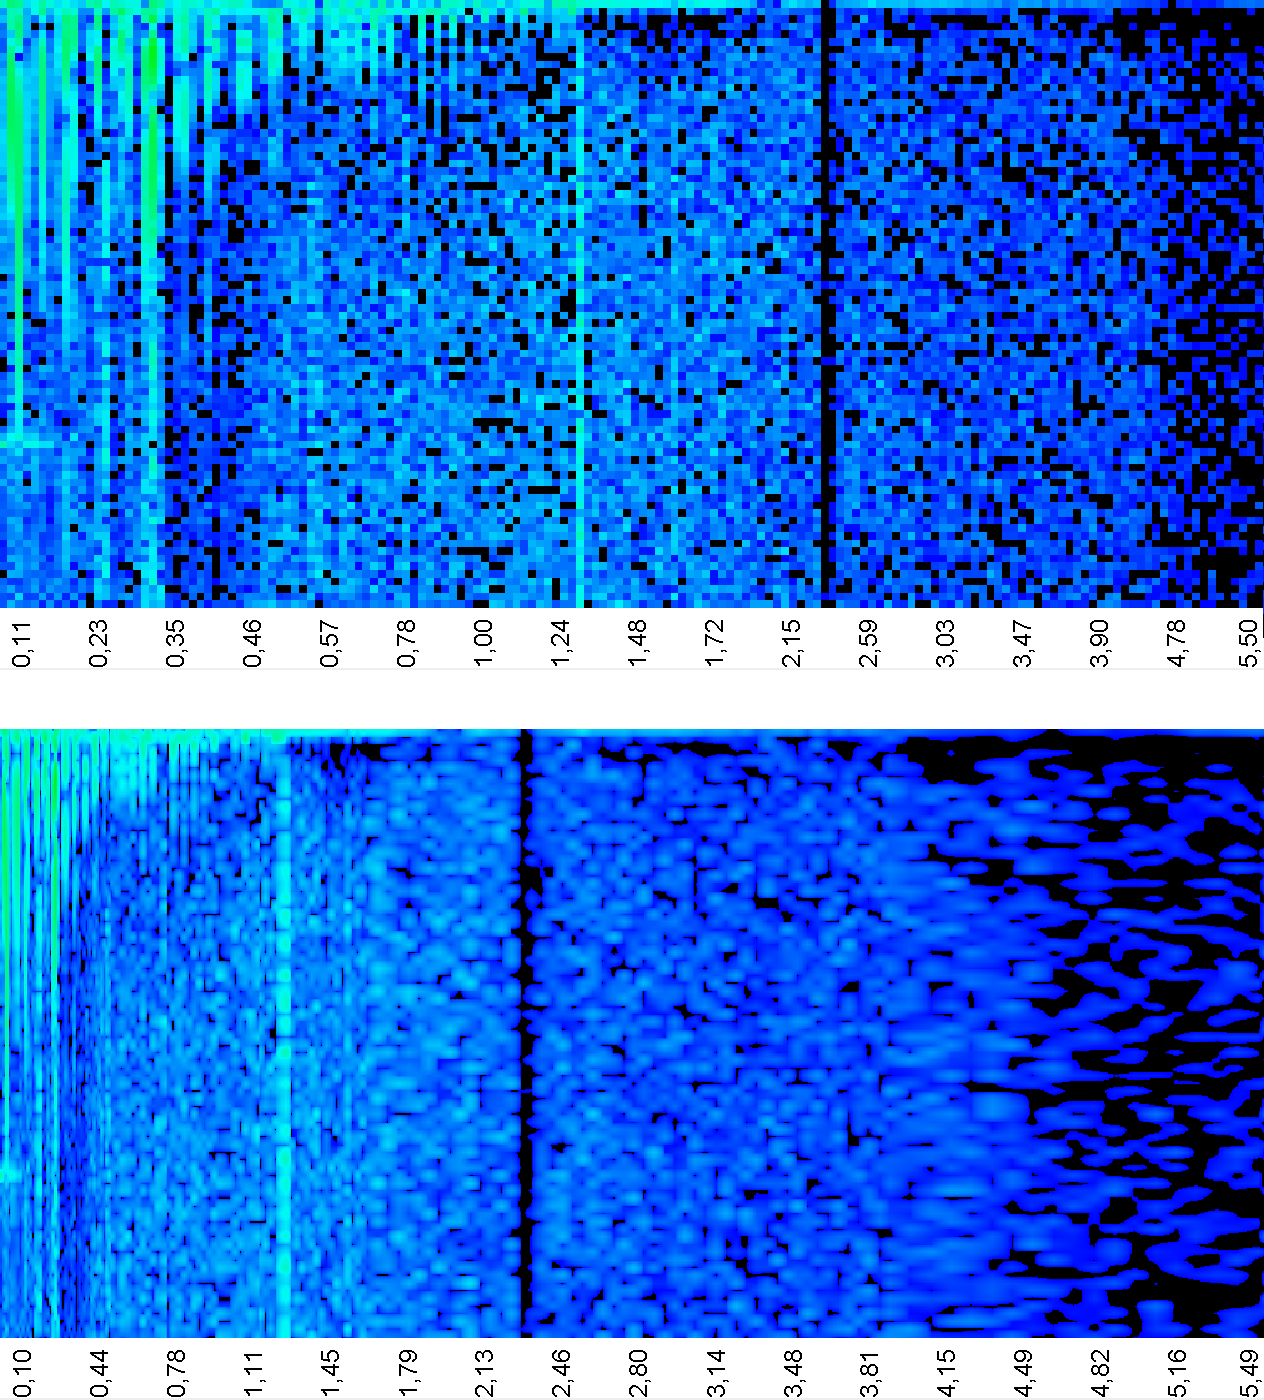
\includegraphics[width=140mm]{images/even_and_uneven_ionogram.png}
	\caption{In the top part of this figure, a ionogram is presented. In the bottom part, an evenly sampled ionogram created from the top one is presented. It is worth notice that the labels of horizontal (frequency) aces of the top ionogram are unevenly distributed. Data from orbit 3874, frame 0 \citep{FTP}.}
	\label{fig:even_uneven_iono}
\end{figure}

\subsection{Features to detect}
We have listed four features of interest - ionospheric echoes (IE), ground echoes (GE), electron plasma oscillations (EPO) and electron cyclotron harmonics (ECH) (in section \ref{ssec:oblique} we have already stated we will omit oblique ionospheric echoes). We detect them based on the fact that they correspond to areas with significantly higher ionogram values than the background. However, ionograms are often very noisy, so it would be difficult (if not impossible) to define a single absolute threshold for telling whether a pixel belongs to a feature or not. 

For verification purposes we manually tagged \n{115495} ionograms from \n{1014} orbits during year 2007. In most of these ionograms we measured the horizontal repeat period (corresponding to EPO) and marked the ionospheric echoes. If no horizontal repetition period was present, we recorded that fact, too. Although being done manually and thus each feature being assessed subjectively, we deduced a rule for distinguishing interesting lines (which are either a feature or a part of a feature). Such line is several pixels wide (cca. 3--\n[px]{20}) and at least that much pixels long (assuming the ionogram has dimension \n{1012}x\n[px]{506}). Values on its skeleton (center line) are at least 10 times higher than those at its border. A line is also allowed to contain ``gaps'', but no more than a third of the line's length in sum. Moreover, every line should contain a value higher than cca. \n{5E-15} (but not all points with higher values belong to a feature). Such definition looks, however, vague. So we add other specific constraints implying from the features we try to detect. 

An EPO or ECH line must be almost straight and must go in exactly vertical or horizontal direction. In addition, one of its ends has to be near the top or left edge of the ionogram (no more than \n[px]{5}). ECH lines usually do not extend to frequencies above \n[MHz]{2.5}. A GE line follows approximately horizontal direction and doesn't have to be straight (due to terrain unevenness; but mostly it is). What should be most helpful is it is placed in the delay time corresponding to the apparent height of the spacecraft over surface (which can be computed). Finally, an IE line has also to be almost horizontal, but it may be substantially curved. It has to appear over the GE (if present).

The statistical tests we conducted\footnote{The application used for these tests is present on the attached CD in folder /programs/statistics along with the data.} on the data from year 2007 show that \n[\%]{95} ionograms with some features have their mean value greater than \n{4.65312E-16}. Ionograms devoid of features have, of course, their mean values even lower than this value (in \n[\%]{74.6} of cases). So we decided this value to be a threshold for telling a ionogram does not contain any features and we will not process it further. This is useful, because the detection algorithms can assume the ionogram either has some features or isn't far from having them.

We also computed other statistical properties of ionograms. We expected the maximum values in ionograms to be a reliable distinguishing mark, and standard deviations, too. As shown in Fig. \ref{fig:data_stats}, neither maxima nor standard deviations show significant differences between the data sets with features and without them. We also made distributions of rather high values (over \n{E-12}) in relation to whether they are a part of a feature. The results shown almost identical distributions, but that can be due to the difficulty of reverse task. E.g. if we save just the period of an EPO, it isn't easily said if a data point belongs to this feature (we try to fit it on whole multiplies of the period, but we don't know the widths of the lines). 

\begin{figure}
	\centering
	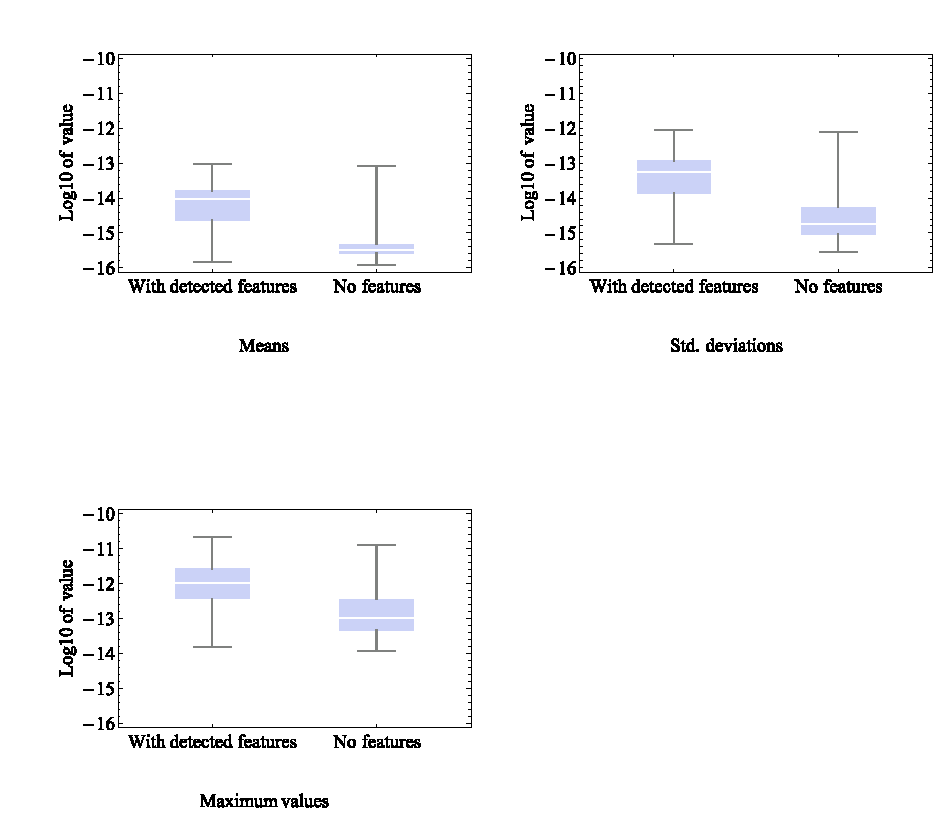
\includegraphics[width=140mm]{images/data_stats.pdf}
	\caption{The distribution of means (top left), standard deviations (top right) and maximum values (bottom left) of individual ionograms from year 2007. The box plots show values for ionograms with features and without features separately. Data from \citep{FTP}.}
	\label{fig:data_stats}
\end{figure}


\section{Title of the second subchapter of the second chapter}
